\documentclass{article}
\usepackage{svg}
\usepackage{hyperref}
\usepackage{amsmath}
\usepackage{amsfonts} 
\usepackage{graphicx}
\usepackage[a4paper,  total={6.75in, 10in}]{geometry}
\usepackage[utf8]{inputenc}


\title{swag di una pandemia con un modello SIRV}
\author{Giulio Pastorello }
\date{Ottobre 2023}

\begin{document}

\maketitle

\section{Il Modello}

\hspace{\parindent} Per descrivere l'andamento della pandemia si è scelto 
di usare un modello SIR al quale è stata aggiunta un quarta 
equazione per rappresentare i vaccinati.\\
Le equazioni che descrivono l'evoluzione della pandemia sono quindi:
\begin{itemize}
\item $S(t)$: "Susceptible". Descrive il numero delle persone non 
malate che non hanno mai contratto l'infezione.
\item $I(t)$: "Infected". Il numero di persone che ad un dato tempo 
t sono malate. 
\item $R(t)$: "Removed". Una volta che una persona è stata 
contagiata, dopo un certo intervallo di tempo viene \textit{rimossa}, 
ovvero guarisce o muore. Si assume che, una volta guariti, 
i soggetti diventino immuni. L'unica possibilità di transizione da 
uno stato all'altro è quindi: $S\xrightarrow{}I\xrightarrow{}R$.
\item $V(t)$: "Vaccinated". Questa equazione è un'aggiunta al modello 
SIR "standard", che prevede solo le prime tre equazioni. 
Anche in questo caso si fa l'assunzione che una persona vaccinata 
non possa più ammalarsi.
\end{itemize}
Il vincolo fondamentale del modello è che la popolazione totale 
sia costante:
$$S(t)+I(t)+R(t)+V(t)=N$$
Questa è un'approssimazione ragionevole se si fa l'assunzione 
che il numero totale di persone che muoiono a causa del virus 
sia trascurabile rispetto alla popolazione totale.
\subsection{Parametri}
Il modello descrive l'andamento della pandemia attraverso alcuni 
parametri:
\begin{itemize} 
\item $\beta \in [0,1]$: questo è interpretabile come la 
\textit{contagiosità} del virus, ovvero la probabilità di 
trasmissione a seguito di un contatto tra un suscettibile e un infetto.
\item $\gamma \in [0,1]$: è l'inverso della durata media di 
un'infezione, che corrisponde alla probabilità di guarigione o morte.
\item $\eta \in \mathbb{N}, \eta < N$: il numero di persone non 
vaccinabili, per motivi medici o personali.
\item $\mu \in\ [0,1]$: rappresenta la velocità delle vaccinazioni.
\item $\xi \in [0,1]$: rappresenta l'efficacia delle vaccinazioni. 
Si usa come fattore moltiplicativo.
\end{itemize}

\subsection{Condizioni Iniziali}
Per studiare la diffusione del virus vengono anche usati come 
condizioni iniziali i seguenti termini:
\begin{itemize}
\item $I_0 \in \mathbb{N}, I_0 < N$: malati al tempo $t = 0$.
\item $V_0 \in \mathbb{N}, V_0 < N $: vaccinati al tempo $t = 0$.
\item $R_0 \in \mathbb{N}, R_0 < N $: rimossi al tempo $t = 0$.
\end{itemize}
Ovviamente si avrà che il numero di suscettibili dall'inizio della 
simulazione ($t = 0$) $S_0$ sarà: \\
$S_0 = N - I_0 - V_0 - R_0$.\\
\subsection{Equazioni}
Usando i parametri descritti sopra, le equazioni differenziali che 
descrivono la diffusione della pandemia sono quindi quattro:\\
\begin{equation} \label{eq::S}
\frac{dS}{dt}(t)= -\beta \frac{S(t)}{N}I(t) - \frac{dV}{dt}(t)
\end{equation}
\begin{equation}\label{eq::I}
\frac{dI}{dt}(t)= \beta \frac{S(t)}{N}I(t) - \gamma I(t)
\end{equation}
\begin{equation}\label{eq::R}
\frac{dR}{dt}(t)= \gamma I(t)
\end{equation}
\begin{equation}\label{eq::V}
\frac{dV}{dt}(t)= \mu\frac{V(t)}{\xi}\left( 1-\frac{V(t)}{\xi(N-\eta)}\right)
\end{equation}
Una simulazione basata su dati rappresentativi dell'Emilia-Romagna
 è mostrata in figura (\ref{fig::SIRV}). 
 Si è usato: popolazione totale $N=4459000$, $\beta=0.05$, 
 $\gamma=0.02$, $I_0 = 530502$, $R_0 = 320000$, $V_0 = 600437$,
 non vaccinabili $\eta = 251042$, 
 velocità vaccinazioni $\mu = 0.05$, efficacia 
 vaccino $\xi= 0.83$.

 \subsection{Curva Logistica}
Per rappresentare la progressione della campagna vaccinale, 
nell'equazione (\ref{eq::V}) si è scelto di usare un'equazione 
logistica generalizzata: $f'(x)=f(x)(1-f(x))$,
che ha come soluzione un sigmoide. Quest'approssimazione è 
ragionevole perché ci si aspettava un inizio più lento dovuto alla 
scarsità di vaccini e all'organizzazione non ancora rodata, 
seguito da una crescita veloce della quantità di persone vaccinate, 
seguito inevitabilmente da una diminuzione dovuta al fatto che le 
persone da vaccinare sono sempre meno. 
COME CAZZO HO STIMATO QUEI PARAMETRI.
Il limite dell'equazione logistica è che usando come numero di 
vaccinati iniziali $\nu = 0$ la campagna vaccinale resta a zero, 
ma partendo da un qualsiasi altro numero si arriverà sicuramente a 
vaccinare tutti i vaccinabili, in un tempo che dipende dalla velocità 
delle vaccinazioni $\mu$. In figura (\ref{fig::vaccinati}) un 
andamento possibile della curva dei vaccinati.\\
\begin{figure}[h!]
\centering
\begin{minipage}[t]{.4\paperwidth}
    \hspace{-10pt}
    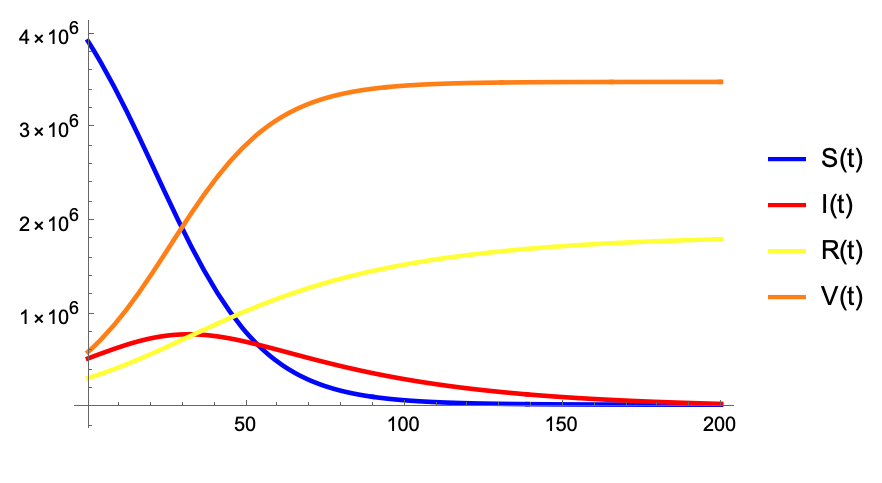
\includegraphics[width=\textwidth]{SIRV.png}
    \caption{\textit{Comportamento del modello SIRV con dati 
    rappresentativi dell'Emilia-Romagna}}
    \label{fig::SIRV}
    \end{minipage}%
\hfill %
\begin{minipage}[t]{.4\paperwidth}
    \hspace{-10pt}
    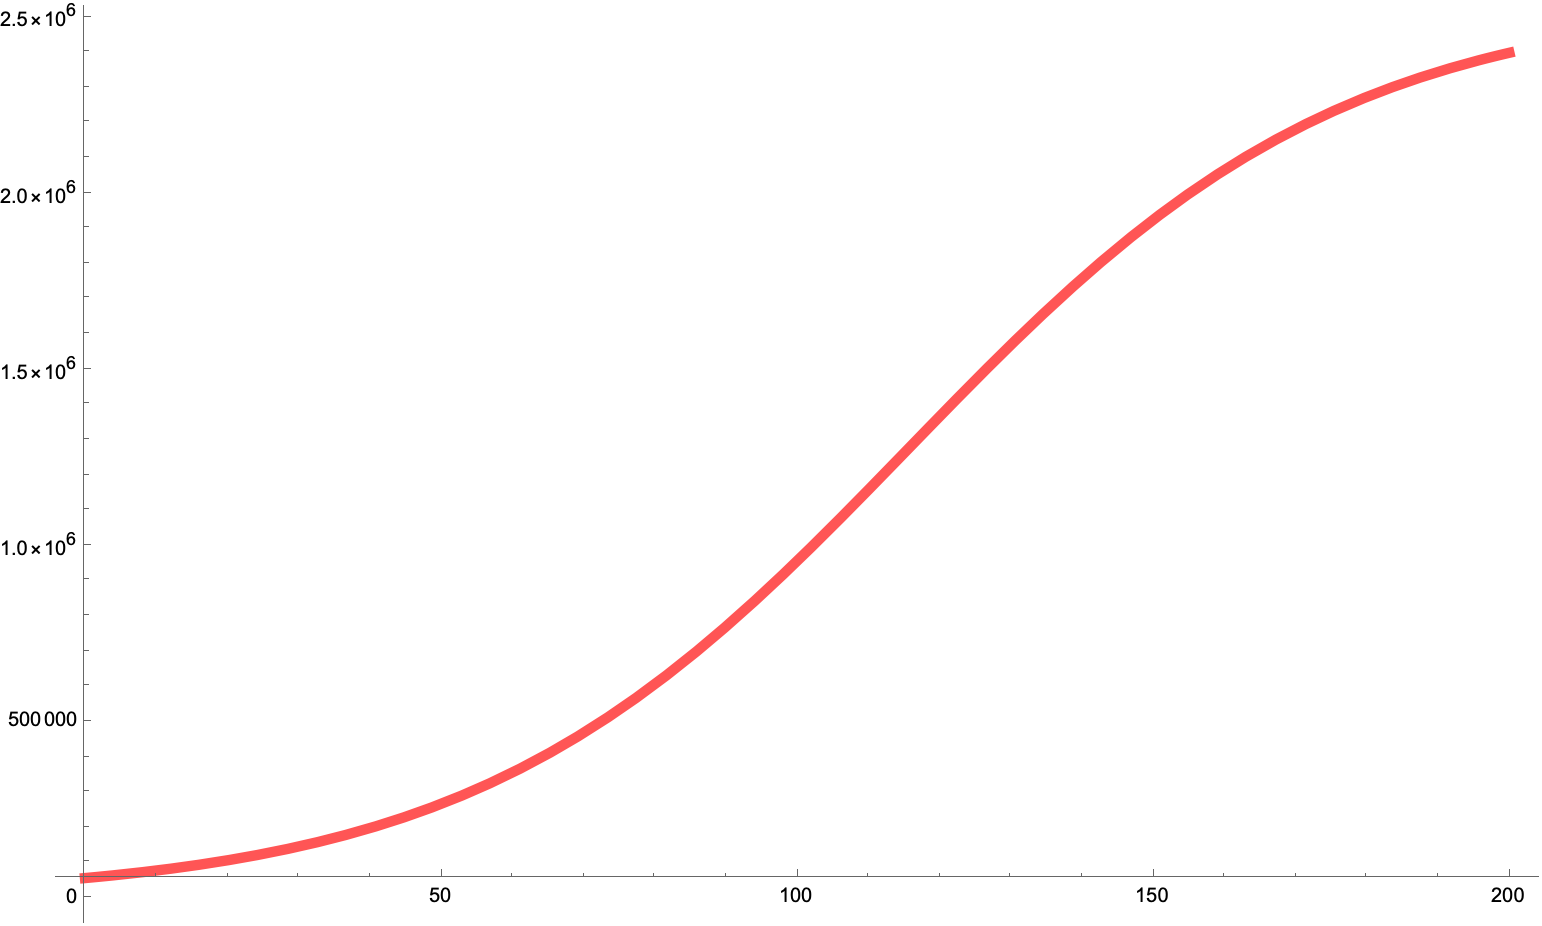
\includegraphics[width=\textwidth]{vaccinati.png}
    \caption{\textit{Curva logistica con $\nu=56980, 
    \mu=0.0274216, \eta=1418957$, e popolazione totale della 
    regione Emilia-Romagna.}}
    \label{fig::vaccinati}
\end{minipage}
\end{figure}
\end{document}
